% Directory
\newcommand{\fighd}{/RECHERCHE/RUPTURES/Exposes/Figures}

% Microarray now constitute a common technique to evaluate DNA and RNA
% abundance within a cell or population of cells. The first lecture will
% focus on high-density array where probes are spread all along the
% genome, regardless of the gene positions. We will consider their use
% for the detection of new genes, protein-DNA interactions or
% chromosomal aberrations.

%====================================================================
\section{High-density (tiling) arrays}
\frame{\frametitle{High-density (tiling) arrays}}
%====================================================================
\subsection{Microarray technology}
%==================================================================== 
\frame{\frametitle{Technology}
  \paragraph{Hybridisation:} complementary single-strands DNA
  molecules:
  $$
  \begin{tabular}{c}
    {\tt $\cdots$ a t g g t a \emphase{t} c a $\cdots$} \\ 
    {\tt $\cdots$ t a c c a t \emphase{c} g t $\cdots$}  
  \end{tabular}
  $$
  \emphase{spontaneously hybridise} when present in the same solution.

  \bigskip\pause
  \paragraph{Microarray:} 
    \begin{itemize}
    \item 'Glass' slide divided into cells $\rightarrow$ '\emphase{array}';
  \item each cell contains copies of a same single-stranded DNA
    fragment: \emphase{'probe'};
  \item each probe is \emphase{associated} with a given gene, SNP,
    species (16S), \dots
  \end{itemize}
  }

%==================================================================== 
\frame{\frametitle{Technology}
  \hspace{.6cm}
  \epsfig{file=\fighd/MicroarrayTech.ps, scale=.55,
    clip=, bbllx=21, bblly=49, bburx=574, bbury=416}
  }

%====================================================================
\subsection{Most popular arrays}
%==================================================================== 
\frame{\frametitle{Most popular arrays}
  \paragraph{Gene expression:} 1 probe (or probset) = 1 gene. \\
  $$
  X_{ij} \propto \left(
    \begin{tabular}{c}
      abundance of gene $i$ transcripts \\
      in sample $j$
    \end{tabular}    \right)
  $$
  $\approx 10^4$ genes in superior organisms.

  \bigskip\bigskip\pause
  \paragraph{SNP arrays:} pair of probes = pair of alleles.  
  $$
  (X_{ij}, Y_{ij}) \propto \left(
    \begin{tabular}{c}
      relative abundance of both alleles of SNP $i$ \\
      in sample $j$
    \end{tabular}    \right)
  $$
  $\approx 10^5$ known SNP in superior organisms.
  }

%====================================================================
\frame{\frametitle{Deeply studied statistical problems}
  \paragraph{Class discovery:} comparison of gene expression profiles
  accross conditions (e.g. times)\\
  $\rightarrow$ clustering

  \bigskip\bigskip
  \paragraph{Class comparison:} comparison of gene expression or
  SNP frequencies between few conditions \\
  $\rightarrow$ multiple testing, FDR, local FDR, etc\dots

  \bigskip\bigskip
  \paragraph{Class prediction:} prediction of a phenotype based on
  gene expression or SNP \\
  $\rightarrow$ classification, variable selection

  \bigskip\bigskip
  \paragraph{Bibliography:} $\approx$ hundreds of papers on each topic.
  }

%====================================================================
\subsection{Tiling arrays}
%==================================================================== 
\frame{\frametitle{Tiling arrays}
  \paragraph{Probes are 'regularly' spaced} along the genome
  $\rightarrow$ \emphase{tiling}. 
  
  \bigskip\bigskip
  \begin{tabular}{lll}
    \paragraph{Question}  & $\rightarrow$ & \paragraph{Hybridized sample} \\
    \\ \pause
    Where are the (unknown) genes? & $\rightarrow$ & All transcripts (RNA) \\  
    \\ \pause
    \hspace{-.3cm}
    \begin{tabular}{p{.5\textwidth}} 
      At which locus does a given protein bind with the chromosome 
    \end{tabular}
    & $\rightarrow$ & 
    \hspace{-.3cm}
    \begin{tabular}{p{.3\textwidth}} 
      Immuno-precipitated chromatin (DNA)
    \end{tabular} \\
    \\ \pause
    \hspace{-.3cm}
    \begin{tabular}{p{.5\textwidth}} 
      Are there copy number variation (CNV) along the genome 
    \end{tabular}
    & $\rightarrow$ & Genomic DNA 
  \end{tabular}
  }

%====================================================================
\section{Signal detection}
\frame{ \frametitle{Signal detection}
  }
%====================================================================
\subsection{Protein-DNA interaction}
%==================================================================== 
\frame{ \frametitle{Chromatin structure}
  \vspace{-0.5cm}
  $$
  \hspace{-0.5cm}
  \begin{tabular}{ll}
    \begin{tabular}{p{.6\textwidth}}
      \paragraph{Chromatin} is the \emphase{strongly structured} complex that
      contains the DNA molecule.

      \\
      \paragraph{Histones} are proteins that constitute the basic bricks
      of this complex, around which the DNA is wrapped.

      \\ 
      This structure 
      \begin{itemize}
      \item has some influence on gene expression (\emphase{accessibility} for
        transcription) 
      \item can be inherited (\emphase{'epigenetics'})
      \end{itemize}
    \end{tabular}
    &
    \hspace{-.5cm}
    \begin{tabular}{p{.4\textwidth}}
      \epsfig{file = \fighd/chromatin-structure.ps, scale=.25, clip=} 
    \end{tabular}
  \end{tabular}
  $$
  }

%==================================================================== 
\frame{ \frametitle{ChIP on chip}
  \paragraph{ChIP = } Chromatin Immuno-Precipitation, aims at
  detecting protein-DNA interactions.
  $$
  \hspace{-0.5cm}
  \begin{tabular}{ll}
    \begin{tabular}{p{.5\textwidth}}
      \paragraph{ChIP-chip:} Probes corresponding to different loci
      are spotted on a glass slide. 
      \begin{itemize}
      \item \emphase{log IP:} DNA fragments interacting with the
        protein of interest (e.g. histone).
      \item \emphase{Input:} whole genomic DNA.
      \end{itemize}
      $$
      \emphase{X = \log(\text{IP1}/\text{IP2})}
      $$
      Non-zero $X$ reveal \emphase{differential protein-DNA
        interaction} between samples 1 and 2.
    \end{tabular}
    &
    \hspace{-.5cm}
    \begin{tabular}{p{.5\textwidth}}
      \epsfig{file = \fighd/Chip-chip.ps, scale=.3, clip=} 
    \end{tabular}
  \end{tabular}
  $$
  }

%====================================================================
\subsection{HMM as a natural modelling}
%==================================================================== 
\frame{\frametitle{HMM as a natural modelling}
  Denoting
  \begin{itemize}
  \item $X_t = \log(\text{IP1}_t/\text{IP2}_t)$ the signal observed
    for probe $i$, $\Xbf = \{X_t\}$, 
  \item $S_t$ its unknown status $\in \{0, 1\}$ or $\{-1, 0, +1\}$,
    $\Sbf = \{S_t\}$, 
  \end{itemize}
  we can assume that \pause
  \begin{itemize}
  \item the $S_t$'s are Markov-dependent:
    $$
    \{S_t\} \sim MC(\pibf), \qquad \pi_{k\ell} = \Pr\{S_t = k |
    S_{i-1} = \ell\} \pause
    $$
  \item the $X_t$'s are independent conditionally to the $S_t$'s: 
    $$
    (X_t |S_t = k) \sim f_k(\cdot) = f(\cdot; \theta_k), 
    \qquad \text{e.g. } f_k = \Ncal(\mu_k, \sigma^2_k).
    $$
  \end{itemize} \pause
  We have to estimate
  $$
  \{\pi_k, \mu_k, \sigma^2_k\}_k
  \qquad \text{and} \qquad
  \tau_{ik}  = Pr\{S_t=k | \Xbf\}
  $$
  }

%==================================================================== 
\frame{\frametitle{Standard inference: E-M}
  Base on the decomposition
  $$
  \log P(\Xbf; \thetabf) = \Esp[\log P(\Xbf, \Sbf; \thetabf)|\Xbf] +
  \Hcal[P(\Sbf|\Xbf; \thetabf)]
  $$

  %\hspace{-.5cm}
  \begin{tabular}{p{.45\textwidth}p{.45\textwidth}}
    \paragraph{M-step:} 
    $$
    \max_{\thetabf} \; \Esp[\log P(\Xbf, \Sbf; \thetabf)|\Xbf]
    $$ 

    \bigskip
    $\rightarrow$ Often manageable (weighted likelihood).
    \pause
    & 
    \paragraph{E-step:} 
    $
    \text{calculate} \quad P(\Sbf|\Xbf; \thetabf). 
    $ 

    \bigskip
    $\rightarrow$ \emphase{Doable in $\Ocal(n)$} via the
    forward-backward algorithm
    \begin{itemize}
    \item Forward: $P(S_t | X_1^t)$;
    \item Backward: $P(S_t | X_1^n)$.
    \end{itemize}
  \end{tabular}

  \pause
  \paragraph{Graphical representation.} 
  $$
  \begin{array}{ccccccc}
    \dots & \fbox{$Z_{i-1}$} & \longrightarrow & \fbox{$Z_i$} &
    \longrightarrow & \fbox{$Z_{i+1}$} & \dots \\ 
    & \downarrow & & \downarrow & & \downarrow & \\     
    \dots & \fbox{$X_{i-1}$} & & \fbox{$X_i$} & & \fbox{$X_{i+1}$} &
    \dots \\ 
  \end{array}
  $$
  }

%==================================================================== 
\frame{\frametitle{Probe classification}
  \paragraph{Aim:} assign a status $\widehat{S}_t$ at each probe.

  \bigskip
  \paragraph{Maximum a posteriori (MAP):}
  $$
  \widehat{S}_t = \arg\max_k P(S_t|\Xbf ; \widehat{\thetabf})
  $$ \pause
 \paragraph{Viterbi algorithm:} provides a most probable path given
  the data
  $$
  \widehat{\Sbf} = \arg\max_{\Sbf} P(\Sbf|\Xbf ; \widehat{\thetabf})
  $$\pause

  \paragraph{First may not be best:} you may have
  \begin{eqnarray*}
    \widehat{\Sbf} = \Sbf_{(1)} & \neq & \Sbf_{(2)} \simeq \dots
    \simeq \Sbf_{(10)} \\
    P(\Sbf_{(1)}|\Xbf ; \widehat{\thetabf}) & \ll & P(\Sbf_{(2)}|\Xbf ;
    \widehat{\thetabf}) + \dots + P(\Sbf_{(10)}|\Xbf ;
    \widehat{\thetabf}).
  \end{eqnarray*}
  \ra Need for an exploration of the space of paths.
  }

%====================================================================
\subsection{ChIP on chip}
%====================================================================
\frame{ \frametitle{Application to histone modification}
  \paragraph{Comparison with genome annotation.} (Mixture vs HMM)

  \bigskip\noindent
  \begin{tabular}{cc}
    \begin{tabular}{p{0.45\textwidth}}
      The probe classification provided by the HMM is more consistent
        with their spatial organisation. \\
      ~\\
      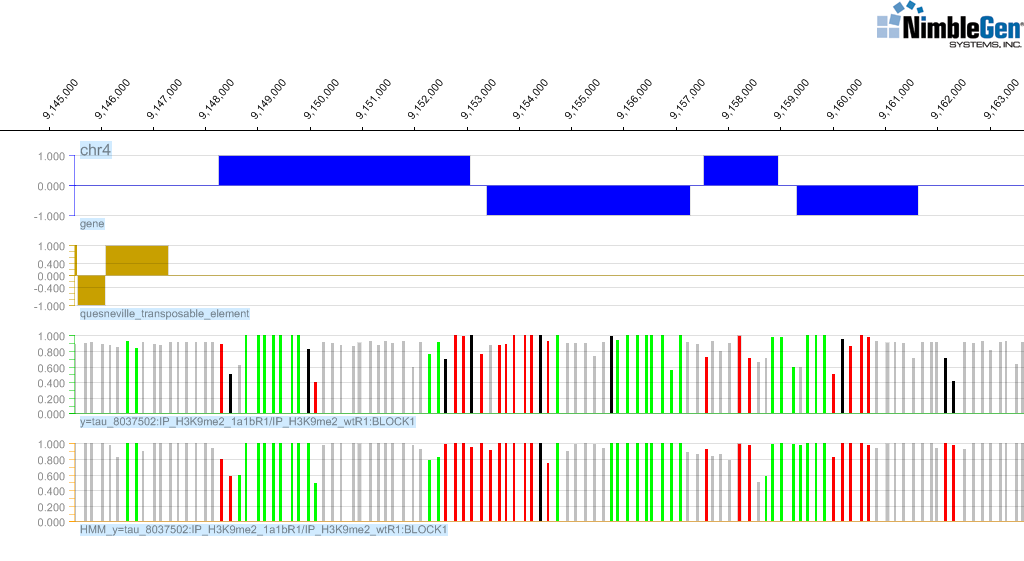
\epsfig{file = \fighd/SignalMap_9145_flagdb_bis.ps,
        width=0.45\textwidth, clip=} \\
      ~\\
    \end{tabular}
    &
    \hspace{-.5cm}
    \begin{tabular}{p{0.45\textwidth}}
      The Methylation mark in META1 is lost in the mutant, mostly in
        the left-end part, near the regulatory region. \\
      ~\\
      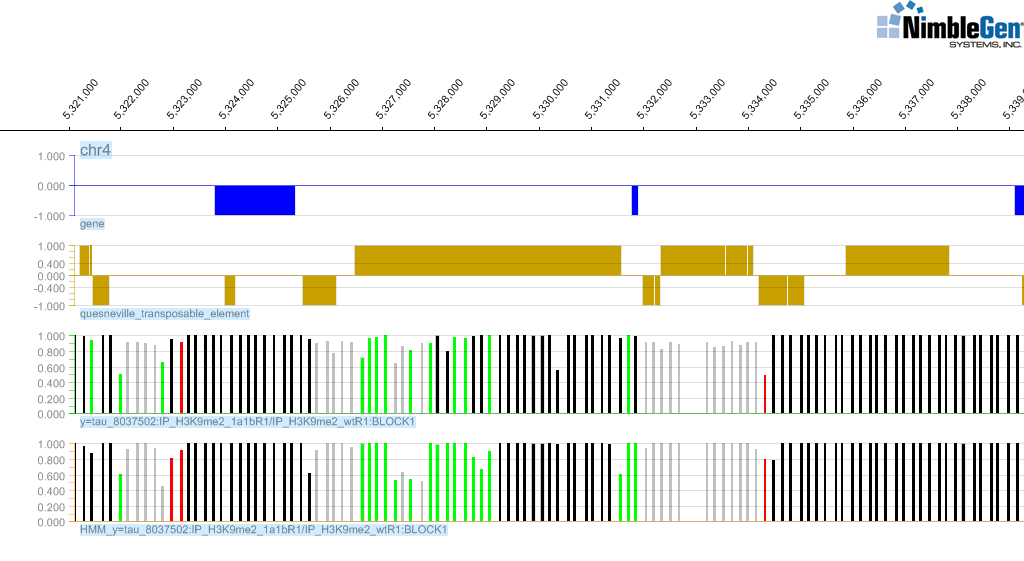
\epsfig{file = \fighd/SignalMap_META1_flagdb_bis.ps,
        width=0.45\textwidth, clip=} \\   
      ~\\
    \end{tabular}
  \end{tabular} \\
  Legend: \textcolor{green}{lost}, \textcolor{red}{enriched},
  normal (source \Refer{Berard})
  }

%====================================================================
\subsection{Gene expression}
%====================================================================
\frame{ \frametitle{Transcriptomic tiling-arrays}
  \paragraph{Sample = Transcripts:} allows to
  \begin{itemize}
  \item measure gene expression;
  \item compare gene expression between samples;
  \item discover \emphase{new genes}
  \end{itemize}

  \bigskip\pause
  \paragraph{Confirming alternative annotation for A. Thaliana:}
  $$
  \epsfig{file = \fighd/Fig-CBerard-Eugene.ps, width=1\textwidth, clip=}
  $$
  \textcolor{blue}{Official annotation} vs \textcolor{purple}{EuGene
    annotation} (source \Refer{C. Berard / FlagDB})
  }

%====================================================================
\frame{ \frametitle{Some refinements}
  \paragraph{Gene classification.} HMM provide a classification of
  probes, that need to be summarised at the gene level:
  $$
  \Pr\{\text{Gene } g \in k | \Xbf\} = \Pr\left\{\bigcup_{t \in
      \Ecal(g)} Z_{tk} = 1\right\} 
  $$
  can be calculated as a combination of 'sub'-forward/backward
  recursions across exons from $\Ecal(g)$:
  $$
  \epsfig{file = \fighd/Fig-CBerard-ProbGene.ps, width=.7\textwidth, clip=}
  $$

  \pause
  \paragraph{Annotation} about the position of known genes can be
  encoded is the distribution of $\Sbf$:
  $$
  \pi^c(k, \ell) = \Pr\{Z_{t+1}=\ell | Z_t=k, C_t=c\}
  $$
  where $C_t$ stands for the annotation of probe $t$.
  }

%====================================================================
\frame{ \frametitle{Transcriptomic tiling-arrays}
  \vspace{-.5cm}
  \begin{tabular}{cc}
    \hspace{-.5cm}
    \begin{tabular}{p{.45\textwidth}}
      \paragraph{Spatial structure vs annotation:} \\
      MAP classification.\\
      \vspace{.35cm}
      Annotation \\
      \vspace{.55cm}
      (Independent) Mixture \\
      \vspace{.55cm}
      HMM \\
      \vspace{.55cm}
      Mixture + Annotation \\
      \vspace{.55cm}
      HMM + Annotation \\
      (source \Refer{Berard})\\
    \end{tabular}
    &
    \hspace{-.5cm}
    \begin{tabular}{p{.6\textwidth}}
      \epsfig{file = \fighd/CBerard-Evry-25.ps,
        width=0.6\textwidth, clip=} \\   

    \end{tabular}
  \end{tabular}
  }

%==================================================================== 
\subsection{Perspective}
\frame{ \frametitle{Perspectives}
  \paragraph{Semi-parametric modelling:} if a reliable null
  ('background') model $\Phi$ is available,
  $$
  X_i \sim (1-S_t) \Phi + S_t F
  $$
  the alternative $F$ can be estimate in a more flexible way. \\
  \ra Semi-parametric mixture; \\
  \ra Averaging of mixture models.
  
  \bigskip\bigskip\pause
  \paragraph{FDR control:} Controlling the number of false detection
  is still desirable. 
  
  FDR control can be achived via intuitive rules based on the
  $\tau_{t0}$ (\refer{SuC08}):
  $$
  \widehat{FDR}(s) = \frac1s \sum_{t=1}^s \tau_{(t)0}.
  $$
  
  }

%====================================================================
\section{Copy number variation (CNV)}
\frame{ \frametitle{Copy number variation (CNV)} 
  }
%==================================================================== 
\subsection{Genomic alterations}
%==================================================================== 
\frame{ \frametitle{Copy number variation in cancer cells} 
  Genomic alterations are associated with (responsible for?) various
  types of cancers.
  $$
  \begin{tabular}{cc}
    Normal cell & Tumour cell \\
    \epsfig{file =
    \fighd/KaryotypeCancer-PH.ps, clip=,
    bbllx=325, bblly=676, bburx=468, bbury=780, scale=.9} 
  
    &
      \epsfig{file =
    \fighd/KaryotypeCancer-PH.ps, clip=,
    bbllx=127, bblly=676, bburx=319, bbury=780, scale=.9} 
    \end{tabular}
  $$
  \refer{Hup08} %\refer{Hup�}{08}
  }

%====================================================================
\frame{ \frametitle{Comparative genomic hybridization (CGH)}
  \begin{tabular}{ccccc}
    \multicolumn{3}{c}{Zoom on CGH profile} & \quad & Karyotype \\
    chrom. 1 & \quad & chrom. 17 \\
                                %   \epsfig{file = \fighd/Karyotype-CGH-PH.ps, clip=,
                                %     bbllx=80, bblly=617, bburx=150, bbury=763, scale=2}
    \epsfig{file = \fighd/Karyotype-CGH-PH.ps, clip=,
      bbllx=80, bblly=617, bburx=150, bbury=700, scale=1.5}
    & &
                                %   \epsfig{file = \fighd/Karyotype-CGH-PH.ps, clip=,
                                %     bbllx=270, bblly=617, bburx=300, bbury=763, scale=2}
    \epsfig{file = \fighd/Karyotype-CGH-PH.ps, clip=,
      bbllx=270, bblly=617, bburx=300, bbury=700, scale=1.5}
    & &
    \epsfig{file = \fighd/Karyotype-CGH-PH.ps, clip=,
      bbllx=364, bblly=617, bburx=485, bbury=763, scale=1}
  \end{tabular}

  \refer{Hup08}
  }


%==================================================================== 
\subsection{Breakpoint detection}
%==================================================================== 
\frame{ \frametitle{A segmentation problem}
  \begin{tabular}{cc}
    Raw profile & Interpretation \\
    \\
    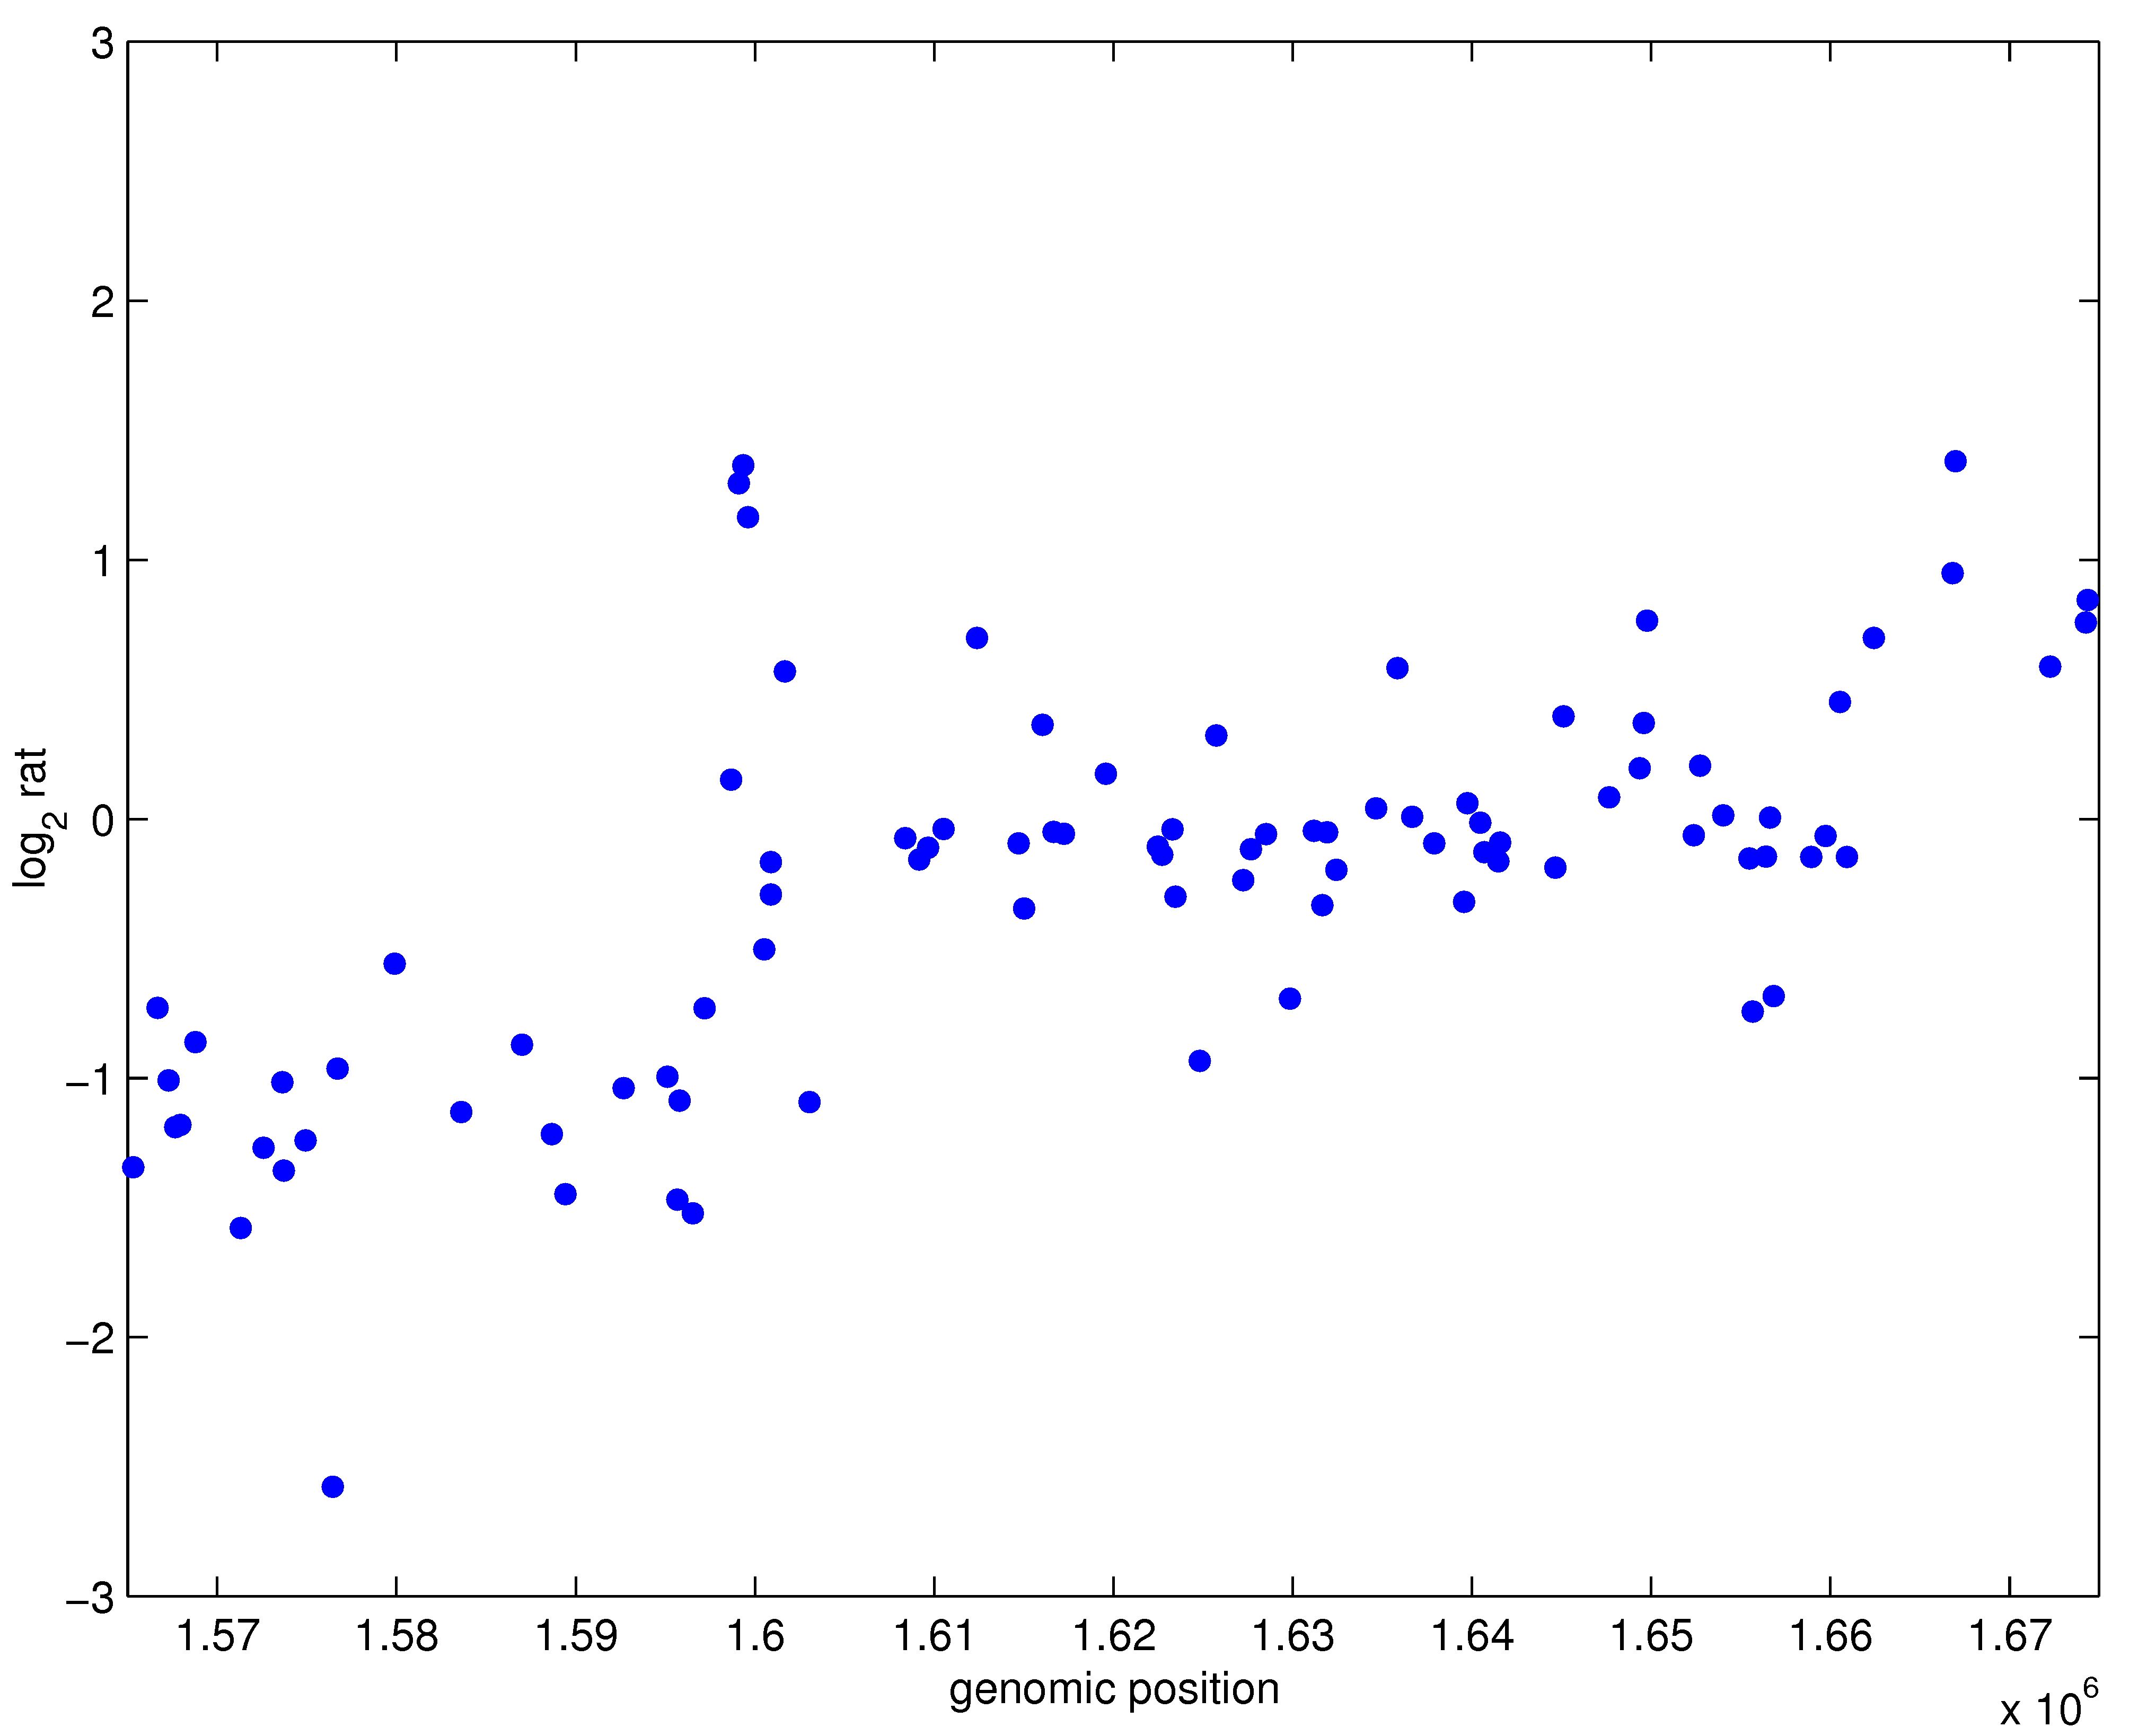
\epsfig{file = \fighd/raw_profile_example.eps, clip=, scale=.325}
      %, bbllx=60, bblly=196, bburx=543, bbury=586}
    &
    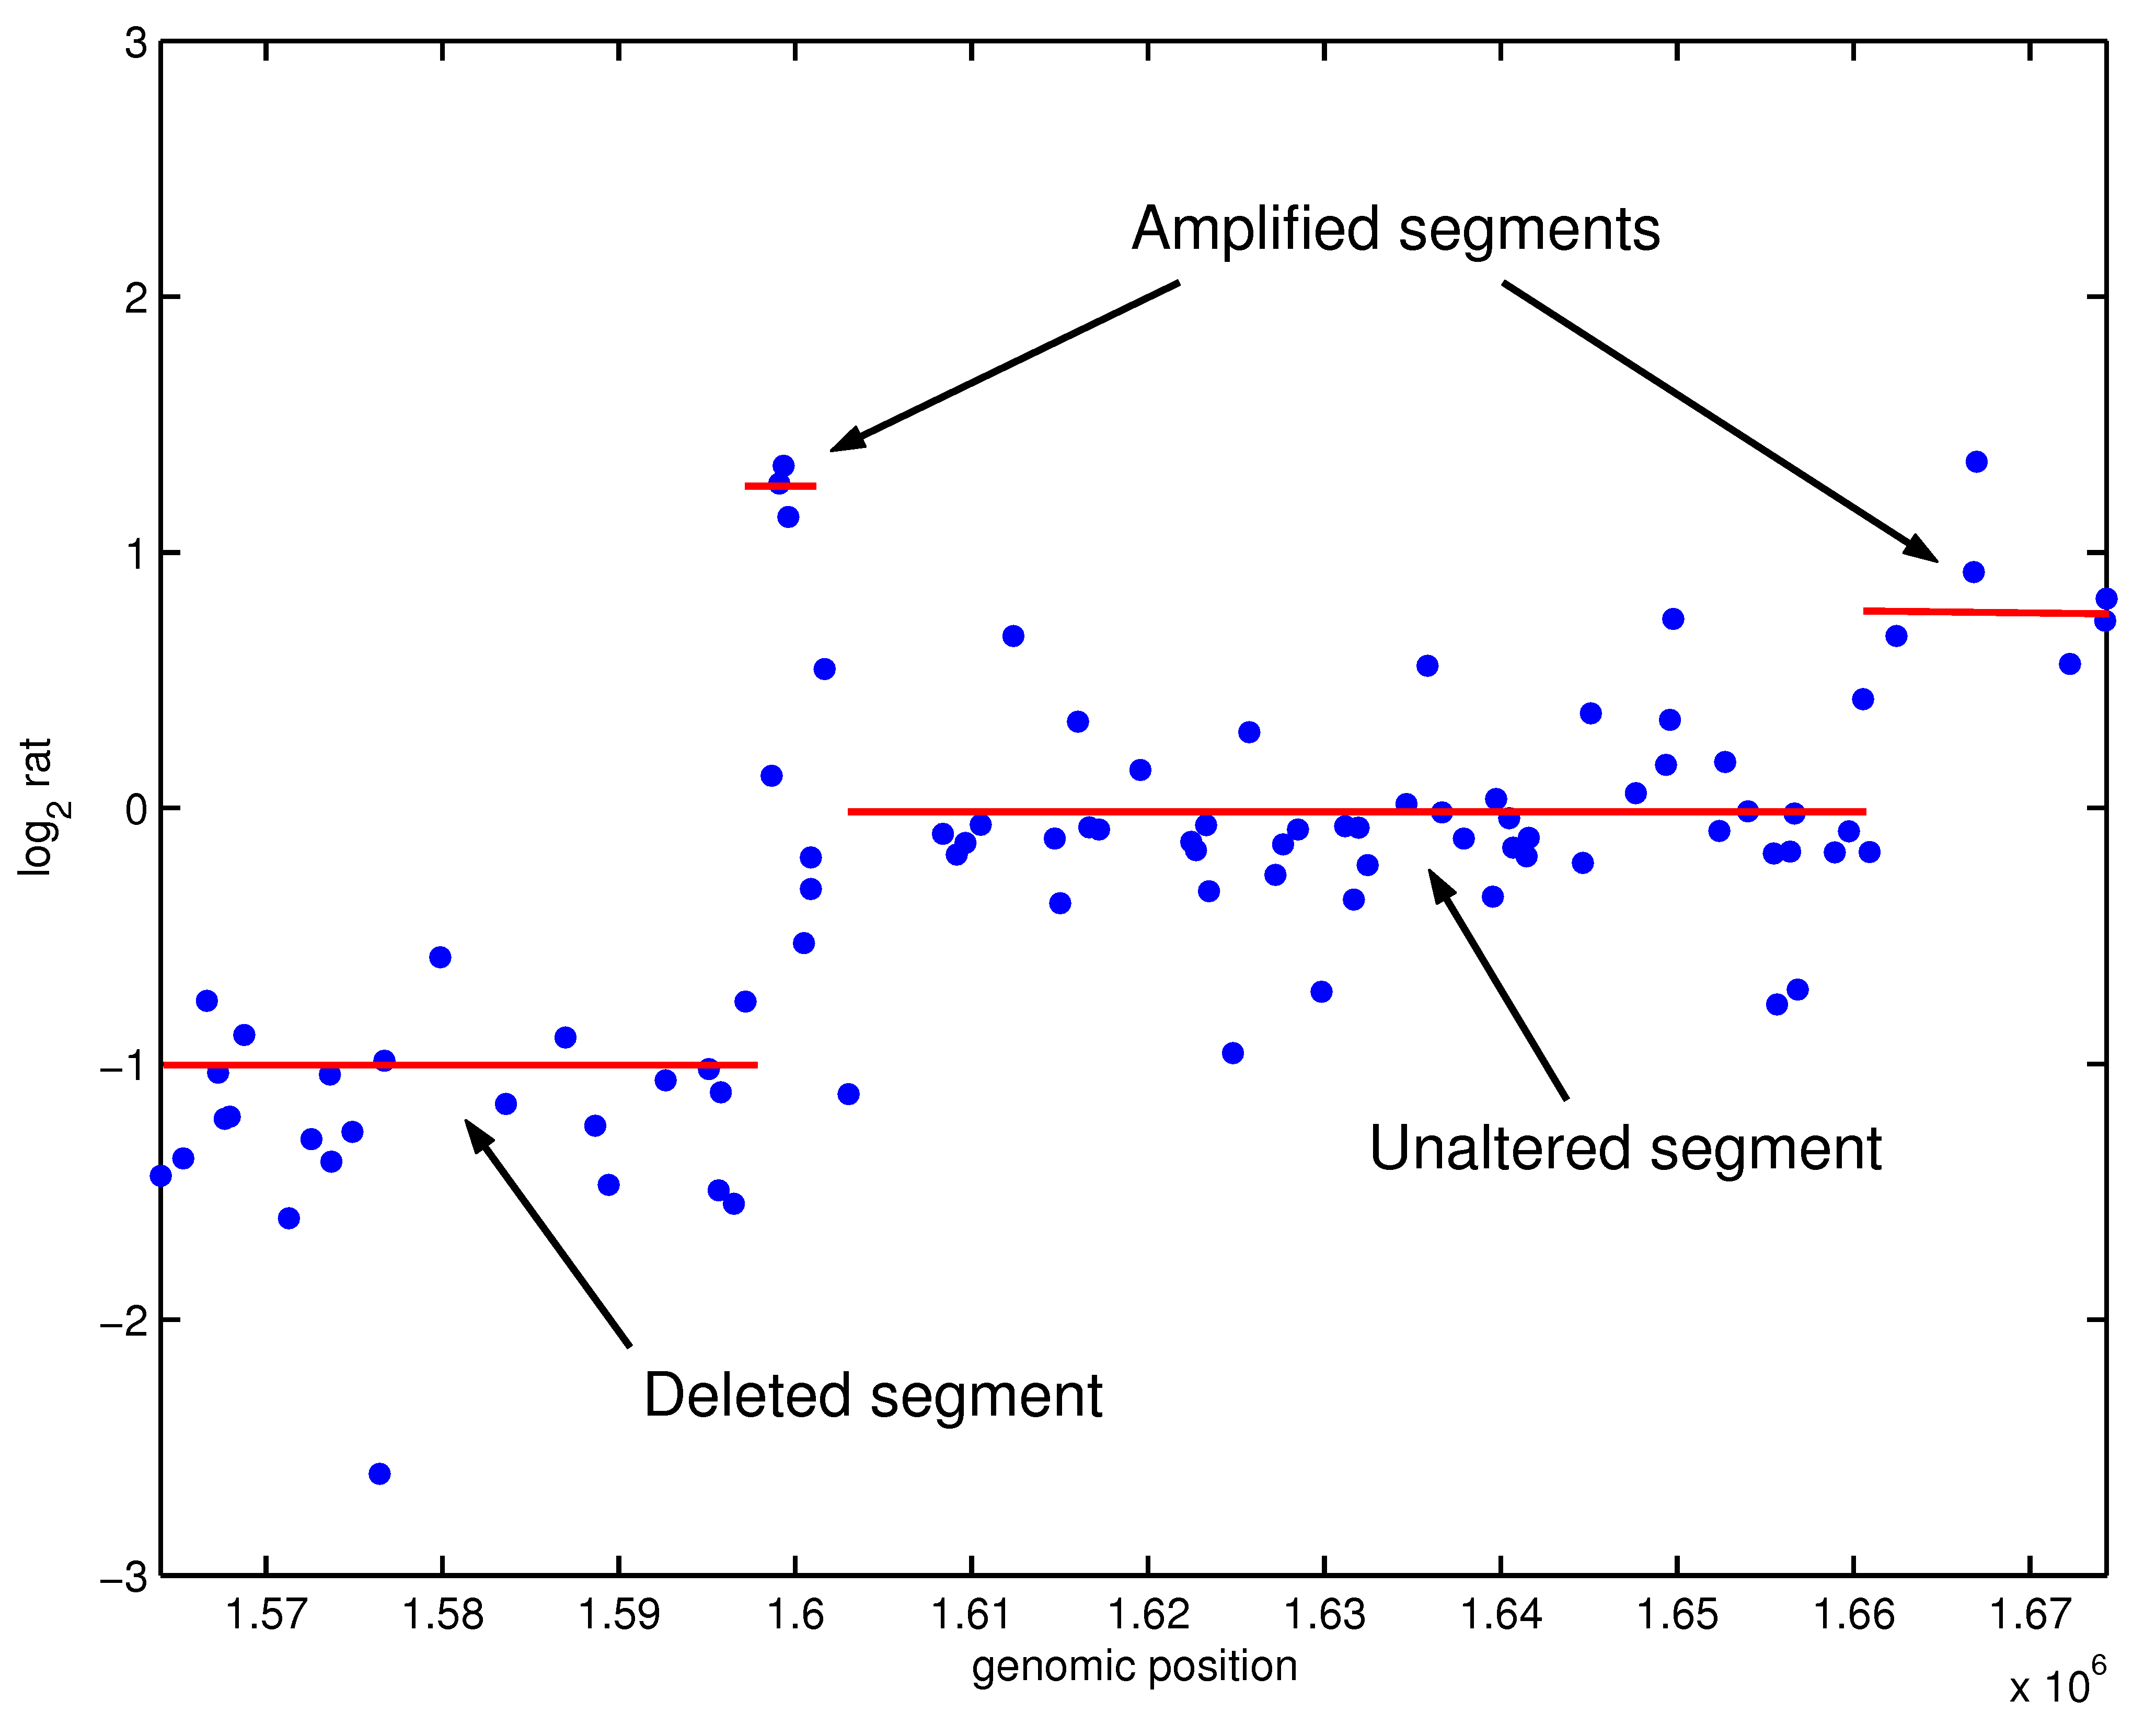
\epsfig{file = \fighd/profile_example.eps, clip=, scale=.325}
      %, bbllx=60, bblly=196, bburx=543, bbury=586}
  \end{tabular} \\
  \refer{Pic05}
  }

%==================================================================== 
\frame{ \frametitle{Change-point model} 
  \emphase{Notations:}
  \begin{itemize}
  \item $K = $ number of segments
  \item $r = $ region $\llbracket \tau_r, \tau^r \rrbracket$; $n_r =$
    length of $r$
  \item $m = $ segmentation: $m = \{r_1, \dots, r_K: \tau_{r+1} =
    \tau^r +1\}$
  \item $Y_t = $ signal at position $t$ ($t \in \llbracket 1, n
    \rrbracket$); $\Ybf = \{Y_t\}$.
  \end{itemize}
  \bigskip
  \emphase{Model:}
  \begin{itemize}
  \item $\{Y_t\}$ independent
  \item $t \in r$: 
    $$
    Y_t \sim p(\cdot | \theta_r)
    $$
  e.g. 
  $$
  p(\cdot|\theta_r) = \Ncal(\mu_r, \sigma^2), \qquad \Ncal(\mu_r,
  \sigma^2_r), \qquad \Pcal(\lambda_r)
  $$
  \end{itemize}
  \refer{PRL05}
  }

%====================================================================
\frame{ \frametitle{Inference}
%==================================================================== 
  \paragraph{Estimation of $\thetabf$ given $m$:} no specific
  problem, can rewritten as a (generallized) linear model:
  $$
  g(\Esp\Ybf) = \Zbf \thetabf.
  $$

  \pause
  \paragraph{General inference:} due to the
  \emphase{discontinuity of $p(\Ybf|m, \thetabf)$} with respect to
  $m$, standard MLE properties do not apply to
  $(\widehat{\thetabf}, \widehat{m})$.  \\
  \ra Inference (e.g.  confidence interval) of the breakpoints is
  not standard.
  
  \bigskip\pause
  \paragraph{Gaussian context:} \Refer{Bai and Perron (1998,
    2003)}\nocite{BaP98,BaP03} proved the consistency of the
  least-square estimates of
  \begin{itemize}
  \item $\widehat{\tau}_k$ at rate $1/n$
  \item $\widehat{\thetabf}$ at rate $1/\sqrt{n}$, with asymptotic normality.
  \end{itemize}
  Other consistency results in \refer{LaM00}.
  }

%==================================================================== 
\subsection{Model selection}
%==================================================================== 
\frame{ \frametitle{Model selection: Choice of $K$}
  \paragraph{Penalised contrast: 2 steps} \pause \\
  %\hspace{-0.5cm}
  \begin{tabular}{p{0.45\textwidth}p{0.5\textwidth}}
    \emphase{1:} Best segmentation within $\Mcal_K$ & 
    $
    \widehat{m}(K) = \arg\min_{m \in \Mcal_K} \ell(\Ybf, m)
    $ \pause \\
    \\ 
    \emphase{2:} Best dimension $K$ & 
    $
    \widehat{K} = \arg\min_{K} \ell(\Ybf, \widehat{m}(K)) + \pen(K)
    $
  \end{tabular}

  \bigskip\pause
  \paragraph{Examples:} \\
  \begin{tabular}{p{0.3\textwidth}p{0.5\textwidth}}
    \refer{Leb05}: & $\pen(K) = f(|\Mcal_K|);$ \\
    \\
    \refer{Lav05}: & $\pen(K) = \beta K.$ \\
  \end{tabular}

  \bigskip
  \begin{itemize} 
  \item \emphase{Constant penalty} within each dimension $\Mcal_K$.
  \item The best model \emphase{$\widehat{m}(K)$ does not depend} on
    the penalty $\pen(K)$.
  \item Some (very sensitive in practice) constants need to be tuned.
  \end{itemize}
  }

%====================================================================
\frame{ \frametitle{Model selection : BIC}
  The standard Laplace approximation used in 
  $$
  \log p(M | \Ybf) = \log \int p(M, \theta | \Ybf) \dd \theta
  \approx \log p(M | \Ybf, \widehat{\theta}) - \frac{\log n}2 \dim(M)
  %=:  \BIC(M)
  $$
  does not hold when the 'model' $M$ refers to the dimension $K$ since
  $$
  \Mcal_K = \bigcup_{m\ \in \Mcal_K} \text{span}(m).
  $$

  \bigskip\pause
  \paragraph{Modified BIC.} Based on uniform prior distribution of the
  breakpoints, \refer{ZhS07} study the behaviour of
  $$
  B_t = S_t - t S_n /n, \quad \text{where } S_t = \sum_{i=1}^t Y_i
  $$
  and derive 
  $$
  \pen(K) = f(|\Mcal_K|) + g\left(\emphase{\sum_{r \in \widehat{m}(K)}
      \log n_r}\right)
  $$
  }

% %==================================================================== 
% \frame{ \frametitle{Example: BT474 cell line, chromosome 1} 
%   \paragraph{Adaptive choice of the number of segments.} :
%   $$
%   \begin{tabular}{cc}
%     Homogeneous variances & Heterogeneous variances \\
%     $\widehat{K} = 10$  segments & $\widehat{K} = 2$ segments \\
%     \epsfig{file = \fighd/bt474_c1_seg_homo_K10.eps, clip=, width=0.4\textwidth} &
%     \epsfig{file = \fighd/bt474_c1_seg_hetero_K2.eps, clip=, width=0.4\textwidth} \\
%   \end{tabular}
%   $$
%   Homogeneous variances result in smaller segments.
%   }

%==================================================================== 
\subsection{Optimal segmentation}
%==================================================================== 
\frame{ \frametitle{Optimal segmentation} 
  For a given dimension $K$, the optimal segmentation has to be found
  within 
  $$
  \Mcal_K = \{m: |m| = K\},
  \qquad |\Mcal_K| = \binom{n-1}{K-1}
  $$ 

  \paragraph{Consequences.}
  \begin{itemize}
  \item \emphase{Exhaustive search} can not be achieved.
  \item \emphase{Dynamic programming} provides maximum likelihood
    $(\widehat{m}, \widehat{\thetabf})$ with complexity $\Ocal(K
    n^2)$.
  \item \emphase{Lasso} criterion can be applied (\refer{TiW08}):
    $$
    \arg\min_m \sum_k \sum_{t \in r_k} (Y_t - \mu_k)^2 + \lambda
    \sum_k |\mu_k - \mu_{k-1}|
    $$
    with linear complexity (\refer{HaL08}).
  \end{itemize}
  }

%==================================================================== 
\frame{ \frametitle{Dynamic programming} 
  \paragraph{Segment cost:} for segment $r = \llbracket i, j
  \rrbracket$, 
  $$
  C(r) = - \log P(Y^r | \widehat{\theta}^r)
  $$
  \bigskip
  \paragraph{Optimal segmentation:} recall $m = \{r_1, \dots, r_K\}$, 
  $$
  \widehat{m} = \arg\max_{m \in \Mcal_K} \sum_k C(r_k)
  $$
  \bigskip
  \paragraph{Optimal segmentation in $K=2$:}
  $$
  S_2(1, n) = \min_{1 < t < n} C(1, t) + C(t+1, n)
  $$
  \bigskip
  \paragraph{Optimal segmentation in $K$:}
  $$
  S_K(1, n) = \min_{K-1 < t < n} S_{K-1}(1, t) + C(t+1, n)
  $$ 
  }

%====================================================================
\frame{ \frametitle{Computational point of view}
  \paragraph{Overall complexity:} Dynamic programming has a
  $\Ocal(n^2)$ complexity because there is a \emphase{quadratic number
    of segments} to be considered.

  \bigskip
  \paragraph{Linear algebra:} The dynamic programming recursion can be
  viewed as a \emphase{scalar product} $\Rightarrow$ For all
    function $F(m)$
  $$
  F(m) = \prod_{r \in m} f(r).
  $$
  Letting $\mathbf{A}: (n+1) \times (n+1)$:
  $$
  \begin{array}{rclll}
    {\bf A}_{ij} & = & f(\llbracket i, j \llbracket ) & \quad & \text{if } 1
    \leq i < j \leq n+1 \\
    & = & 0 & & \text{otherwise.}
  \end{array}
  $$
  Then, 
  $$
  \sum_{m \in \Mcal_k(\llbracket 1, j\llbracket)} F(m) = (\mathbf{A}^k)_{1,j}
  $$
  and \emphase{all terms} for $1 \leq k \leq K$, $1 \leq j
  \leq n+1$, can be computed in \emphase{$O(K n^2)$}.  
  }


%==================================================================== 
\subsection{Exploring the segmentation space}
%====================================================================
\frame{ \frametitle{Exploring the segmentation space: Bayesian framework}
  \vspace{-1cm}
  \begin{description}
  \item[$p(K) = $] prior of dimension $K$;
  \item[$p(m|K) = $] prior of segmentation $m$ given dimension $K$,
    $$
    \text{for example:} \qquad
    p(m|K) = 1 \left/ |\Mcal_K| \right.
    $$
    that is, \emphase{uniform prior} within each dimension;
  \item[$p(m) = $] prior of segmentation $m$,
    $$
    \text{for example:} \qquad
    p(m) \propto \prod_{r \in m} n_r
    $$
    that favours \emphase{regularly spaced} change-points
    ($\rightarrow$ implicit prior on $K$);
  \item[$p(\theta|m) =$] prior of $\theta$ given segmentation $m$.
  \end{description}
  \refer{RLR09}
  }

%==================================================================== 
\frame{ \frametitle{Computing huge sums}
  \paragraph{Under a factorisation assumption:}
  $$
  p(m) = \prod_{r \in m} f(r), 
  \quad
  p(\theta|m) = \prod_{r \in m} f(\theta_r) 
  \quad
  p(\Ybf|m, \theta) = \prod_{r \in m} f(Y^r, \theta_r) 
  $$
  (not true for homoscedastic models), sums can be rewritten as
  $$
  \sum_{m \in \Mcal_K} f(m) = \sum_{m \in \Mcal_K} \prod_{r \in m} f(r)
  $$

  \bigskip\pause
  \paragraph{Total probability:}
  $$
  p(\Ybf|K) = \sum_{m \in \Mcal_K} \prod_{r\in m} \int p(Y^r|\theta_r) p(\theta_r)
  \dd \theta_r = \sum_{m \in \Mcal_K} \prod_{r\in m} p(Y^r)
  $$

  \pause
  \paragraph{Localisation of the $k$-th breakpoint:}
  \begin{eqnarray*}
    \Pr\{\tau_k = t | K, \Ybf\} & \propto & \left(\sum_{m \in \Mcal_k(1, t)} \prod_{r
    \in m} p(Y^r)\right) \left(\sum_{m \in \Mcal_{K-k}(t+1, n)} \prod_{r
    \in m} p(Y^r)\right)
  \end{eqnarray*}
%   \emphase{Conjugate priors.} $\theta^0_r =$ parameter
%     of the prior $p(\theta_r)$
%     $$
%     f(Y^r; \theta^0_r) = \int p(Y^r|\theta_r) p(\theta_r; \theta^0_r) \dd_r
%     \quad \text{has an explicit form.}
%     $$
%     Avoids the Laplace approximation: \\
%     $\rightarrow$ regularity conditions \emphase{are fulfilled} for
%     any segmentation $m$, \\
%     $\rightarrow$ but the asymptotic framework does not apply to small regions.
  }

%====================================================================
\frame{ \frametitle{Exploring the segmentation space}
  We are hence able to compute \pause
  \begin{itemize}
  \item The probability that there is a \emphase{breakpoint at
      position $t$}:
    $$
    \Pr\{\exists k: \tau_k = t | \Ybf, K\} = \sum_{k=1}^K \Pr\{\tau_k = t
    | K\}
    $$ \pause
  \item The probability for a \emphase{segment $r = \llbracket t_1,
      t_2 \llbracket$ to be part of segmentation}
    $$
    \Pr\{r \in m | \Ybf, K\} = \sum_{k=1}^K \Pr\{\tau_k=t_1, \tau_{k+1}=t_2
    | \Ybf, K\};
    $$ \pause
  \item The \emphase{posterior entropy of $m$} within a dimension:
    $$
    \Hcal(K) = - \sum_{m \in \Mcal_K} p(m|\Ybf, K) \log p(m|\Ybf, K) 
    $$\pause
  \end{itemize}   
  \paragraph{Similar to} an algorithm proposed by \refer{Gue07} in the HMM
  context with known parameters.

 }

%====================================================================
\frame{ \frametitle{A CGH profile: $K = 3, 4$}
  \vspace{-.25cm}
  \begin{tabular}{lll}
    \hspace{-0.5cm}
    \begin{tabular}{p{0.2\textwidth}} Optimal segmentation \end{tabular}
    &
    \hspace{-0.5cm}
    \begin{tabular}{l}
      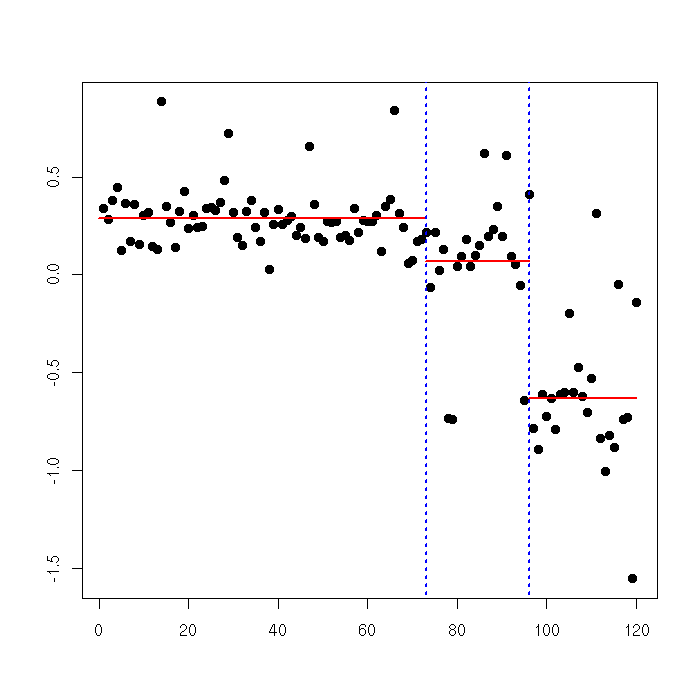
\includegraphics[width=0.35\textwidth, height=0.3\textheight,
      clip=]{\fighd/CopyNumberChr10_BIC}   
    \end{tabular}
    &
    \hspace{-0.5cm}
    \begin{tabular}{l}
      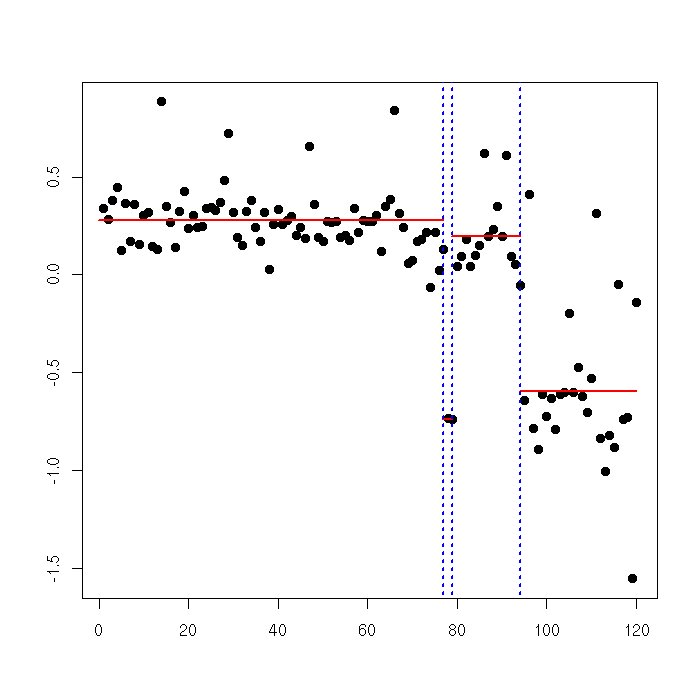
\includegraphics[width=0.35\textwidth, height=0.3\textheight,
      clip=]{\fighd/CopyNumberChr10_ICL}  
    \end{tabular} \\ 
    \hspace{-0.5cm}
    \begin{tabular}{p{0.2\textwidth}} Breakpoint position \end{tabular}
    &
    \hspace{-0.5cm}
    \begin{tabular}{l}
      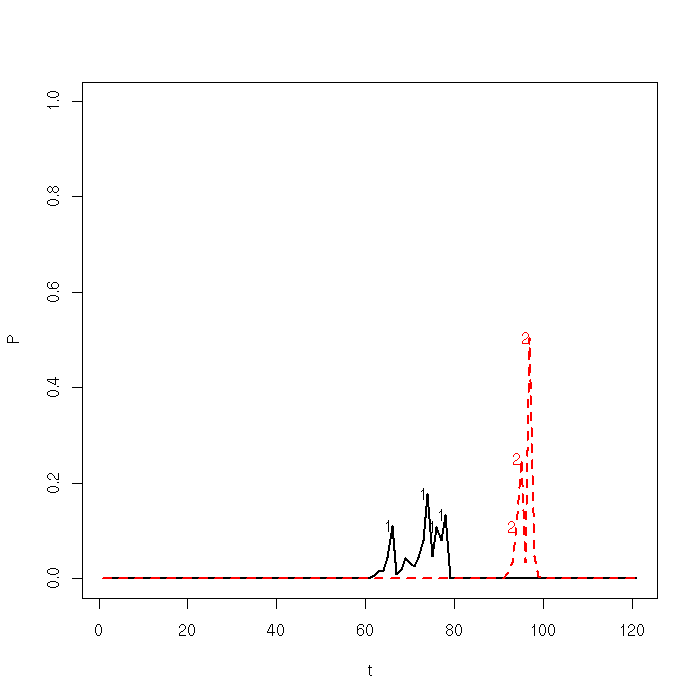
\includegraphics[width=0.35\textwidth, height=0.3\textheight,
      clip=]{\fighd/CopyNumberChr10_ProbaBIC}   
    \end{tabular}
    &
    \hspace{-0.5cm}
    \begin{tabular}{l}
      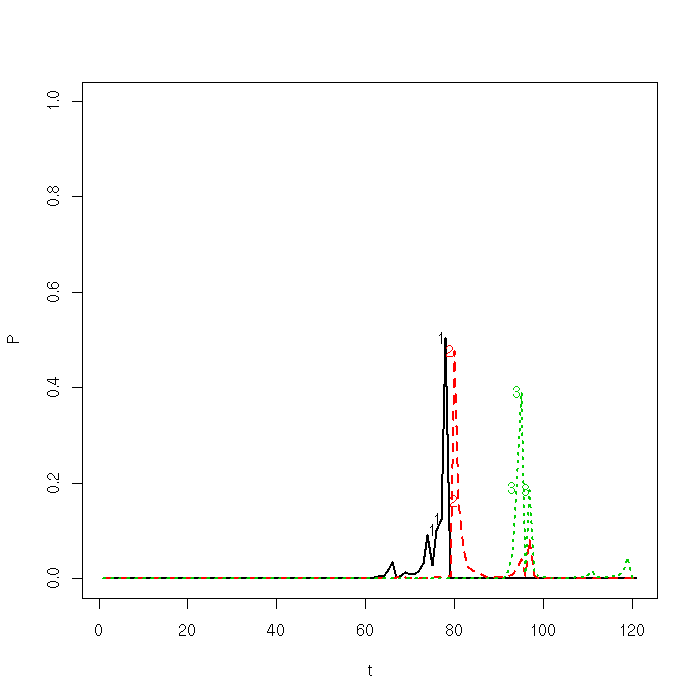
\includegraphics[width=0.35\textwidth, height=0.3\textheight,
      clip=]{\fighd/CopyNumberChr10_ProbaICL}  
    \end{tabular} \\ 
    \hspace{-0.5cm}
    \begin{tabular}{p{0.2\textwidth}} Segment probability \end{tabular}
    &
    \hspace{-0.5cm}
    \begin{tabular}{l}
      \vspace{-.5cm}
      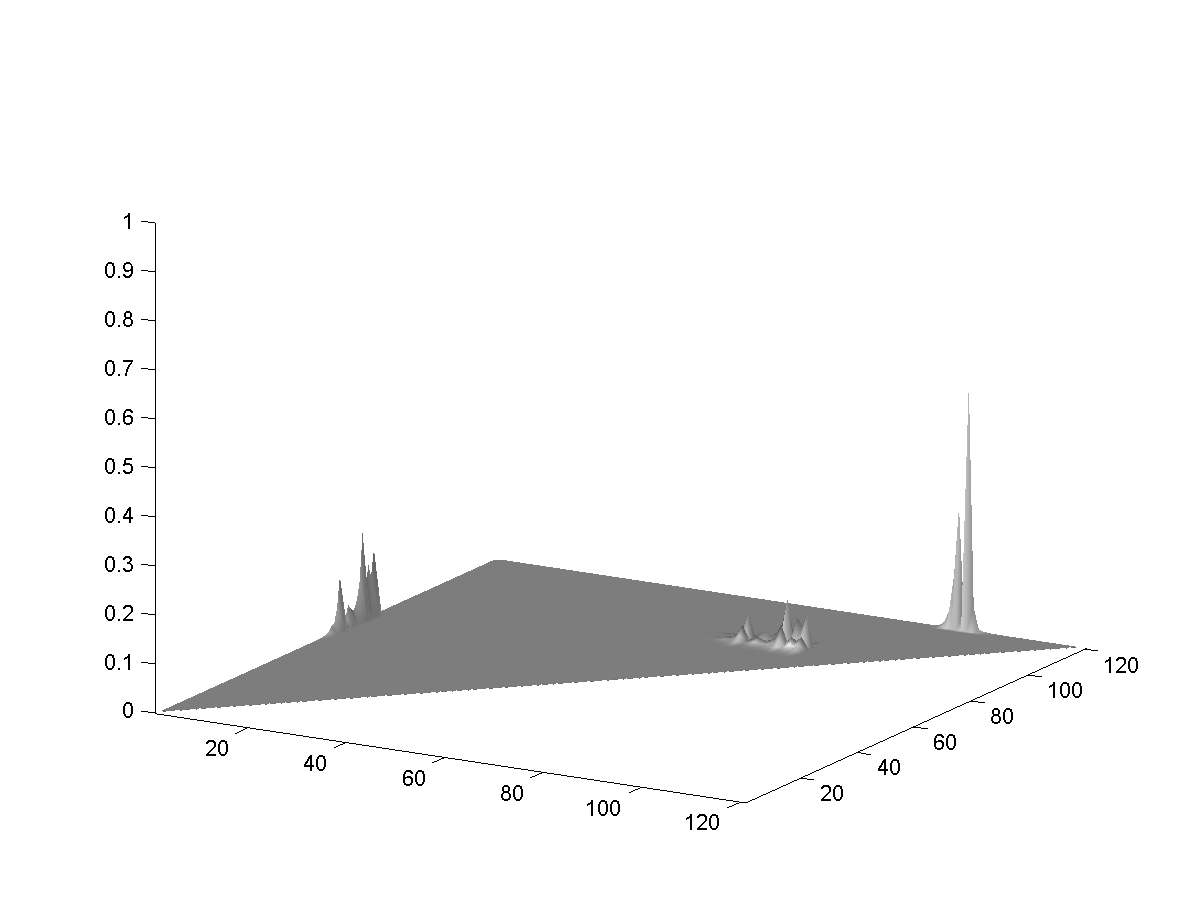
\includegraphics[width=0.35\textwidth, height=0.3\textheight,
      clip=]{\fighd/ProbSeg-BIC}     
    \end{tabular}
    &
    \vspace{-.5cm}
    \begin{tabular}{l}
      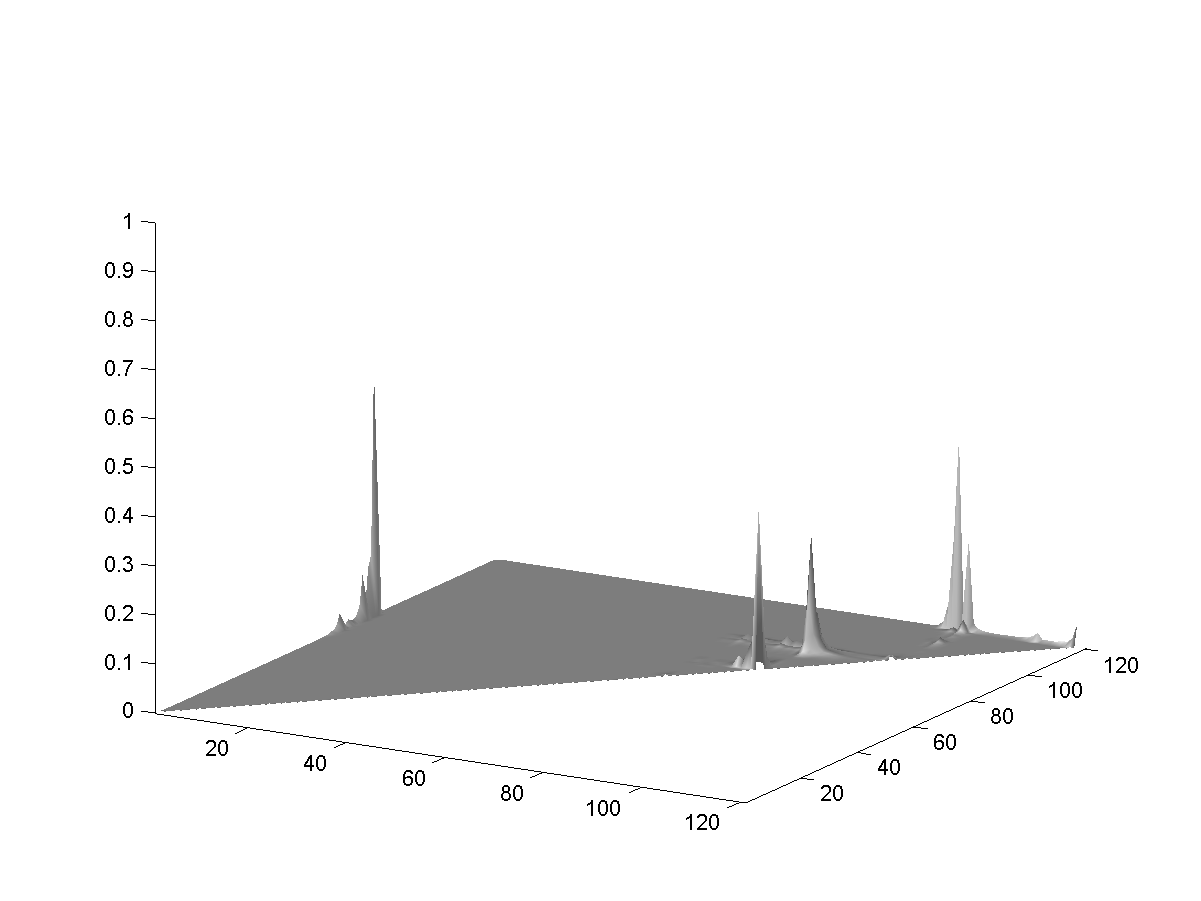
\includegraphics[width=0.35\textwidth, height=0.3\textheight,
      clip=]{\fighd/ProbSeg-ICL}   
    \end{tabular} 
  \end{tabular}
  }

%====================================================================
\frame{ \frametitle{Back to model selection: Exact BIC}
  The conditional probabilities of the dimension and of the
  segmentation also involve 'integral' sums.

  \bigskip
  \paragraph{Choice of $K$.}
  $$
  \BIC(K) = \log p(\Ybf, K) = \log \left[\emphase{\sum_{m \in
        \Mcal_K}} p(m) \int p(\Ybf | m, \theta) p(\theta |m) \dd
    \theta \right].
  $$
  \bigskip\pause
  \paragraph{Choice of $m$.}
  $$
  \BIC(m) = \log p(\Ybf, m) = \log \left[p(m) \int p(\Ybf | m,
    \theta) p(\theta |m) \dd \theta \right]
  $$
  where $p(m)$ must be normalised so that
  $$
  \sum_K \emphase{\sum_{m \in \Mcal_K}} p(m) = 1.
  $$
  }

%====================================================================
\frame{ \frametitle{Exact ICL criterion}
  \emphase{Incomplete data model context} (mixture model):
  \begin{itemize}
  \item \refer{BCG00} add an entropy term $\Hcal(K)$ to the $\BIC(K)$
    penalty
  \item $\Hcal(K)$ accounts for the reliability of the prediction of
    the unknown variable.
  \end{itemize}
  \bigskip \pause
  \emphase{Segmentation context.}
  \begin{itemize}
  \item Change-point positions can be view as unknown variables.
  \item For a given dimension $K$, it is desirable that the best
    segmentation clearly outperforms the others:
    $$
    \text{for any } m \in \Mcal_K \setminus \{\widehat{m}(K)\}:
    \quad p(\widehat{m}(K)|\Ybf) \gg p(m | \Ybf).
    $$
  \item This can be measured by the posterior entropy $\Hcal(K)$
  \end{itemize}
  \bigskip
  \emphase{ICL criterion:}
  $$
  \ICL(K) = \log \sum_{m \in \Mcal_K} p(\Ybf, m) - \Hcal(K)
  $$
    }

%====================================================================
\frame{ \frametitle{Comparison BIC/ICL: Simulation study}
  \begin{columns}
    \begin{column}{0.45\linewidth}
      \emphase{Simulations: } Poisson signal with alternating
      means $\lambda_0$ and $\lambda_1$, $n = 100$. \\
      \bigskip \emphase{Criterion} = \% of recovery of the true number
      of segments ($K =
      5$). \\
      \bigskip
      \begin{itemize}
      \item $\BIC(m)$ achieves (much) better performances than
        $\BIC(K)$
      \item $\ICL(K)$ outperforms both $\BIC(K)$ and $\BIC(m)$.
      \end{itemize}
    \end{column}
    
    \begin{column}{0.45\linewidth}
      \begin{tabular}{c}
        \textcolor{green}{$\BIC(K)$} \quad \textcolor{red}{$\BIC(m)$} \quad
        \textcolor{blue}{$\ICL(K)$} \\
        ~\\
        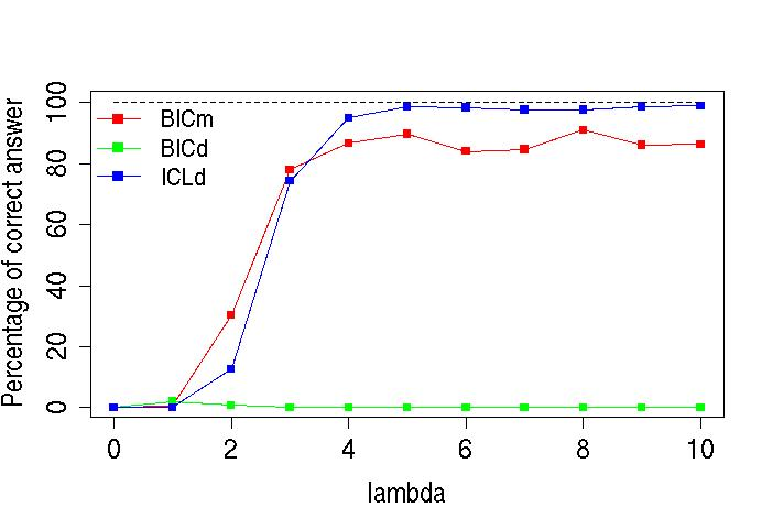
\epsfig{file=\fighd/ICLvsBIC.ps, clip=, bbllx=50, bblly=60,
          bburx=545, bbury=340, width=5cm, height=5cm} \\
        $\lambda_1 - \lambda_0$ ($\lambda_0 = 1$)
      \end{tabular}
    \end{column}
  \end{columns}
 }

%====================================================================
\frame{ \frametitle{}
  \vspace{-1cm}
  $$
  \begin{tabular}{cc}
    \begin{tabular}{c}
      \emphase{\large Back to the example} \\
      \epsfig{file=\fighd/CopyNumberChr1_Alone.ps, 
        bbllx=38, bblly=40, bburx=565, bbury=385, width=4.25cm, height=2.25cm,
        clip=} \\
      \\
      $\BIC(K) \rightarrow \widehat{K} = 10$ \\
      \epsfig{file = \fighd/BIC2_NP.ps,
      width=5cm, height=2.5cm, clip=} \\
    \end{tabular}
    &
    \begin{tabular}{c}
%       \\
%       $\ICL(K) = f[\BIC(K)]$ \\
%       \epsfig{file=\fighd//BICandEntropy.ps,
%       clip=, scale=0.25, bbllx=38, bblly=40, bburx=565, bbury=385}    
      $\BIC(m) \rightarrow \widehat{K} = 3$ \\
%      \epsfig{file = \fighd/BIC_NP.ps,
      \epsfig{file = \fighd/ICL_NP.ps,
      width=5cm, height=2.5cm, clip=} \\
      \\
      $\ICL(K) \rightarrow \widehat{K} = 4$ \\
%      \epsfig{file = \fighd/ICL_NP.ps,
      \epsfig{file = \fighd/BIC_NP.ps,
      width=5cm, height=2.5cm, clip=} \\
    \end{tabular}
  \end{tabular}
  $$
  When $K$ exceeds the 'true' dimension, all segmentations
  nested within the 'true' one have a high posterior probability,
  which increases the entropy. 
}

%==================================================================== 
\subsection{Perspectives}
%==================================================================== 
\frame{ \frametitle{Multiple profile analysis}
  \paragraph{Joint segmentation of multiple profiles:} simultaneous analysis
    of multiple profile allows to account for (\refer{POA09})
    \begin{itemize}
    \item available covariates (e.g. GC probe content),
    \item possible technological biases.
    \end{itemize}

    \pause
    Linear (mixed model) provide a natural framework:
    $$
    \Ybf = \underset{\text{covariates}}{\Xbf \thetabf} +
      \underset{\text{segmentation}}{\Tbf \mubf}  +
        \underset{\text{random technical effect}}{\Zbf \Ubf} + \Ebf
    $$
    E-M algorithm allow to use standard segmentation tools.

    \bigskip\bigskip\pause
    \paragraph{Looking for recurrent aberrations.} When considering as
    set of patients with similar disease, recurrent aberrations have to
    be found:
    \refer{BlV09}, \Refer{R. and Stefanov, 08}\nocite{RoS08}
    }

%==================================================================== 
\frame{ \frametitle{Loss of heterozygoty (LOH).}
  Genomic alterations lead to abnormal allele frequencies:
  \begin{itemize}
  \item Deletion then duplication creates long homozygote regions;
  \item CNV create non-standard allele frequencies, i.e. $\notin \{0,
    .5, 1\}$.
  \end{itemize}

  $$
  \epsfig{file = \fighd/PMS09-GenomeBiol-fig1a-Chr1-2.ps,
    width=.6\textwidth, height=.4\textheight} 
  $$
  (source \refer{PMS09}). \\
  \ra Segmentation in both CNV and allele frequencies allows to trace
  back rearrangement history.
  }

%%% Local Variables: 
%%% mode: latex
%%% TeX-master: "StatSud"
%%% End: 
